\section{Remarks to Clustering}

\mode<presentation>{
\begin{frame} 
    \begin{center} \huge
        \secname
    \end{center}
    \begin{center}
		No relationships between clusters
    \end{center}
\end{frame}
}

\subsection{K-means Sinusoid example}

\begin{frame}{\subsecname}

Consider the following 2-D data and applying K-means with $M=7$ prototypes.

\begin{minipage}{0.45\textwidth}
\begin{center}
	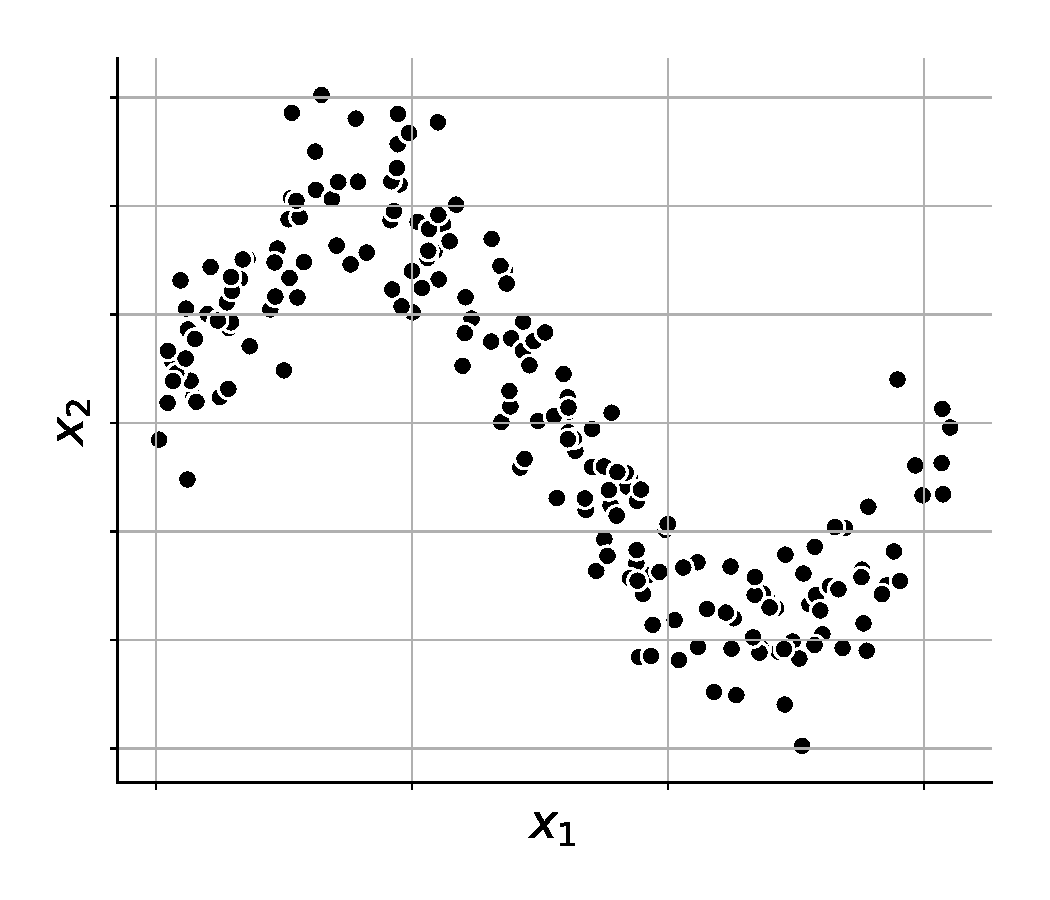
\includegraphics[width=0.8\textwidth]{img/sin_data}
	\notesonly{\captionof{figure}{2D points describing a sinusoid.}}
\end{center}
\end{minipage}
\begin{minipage}{0.45\textwidth}
\begin{center}
	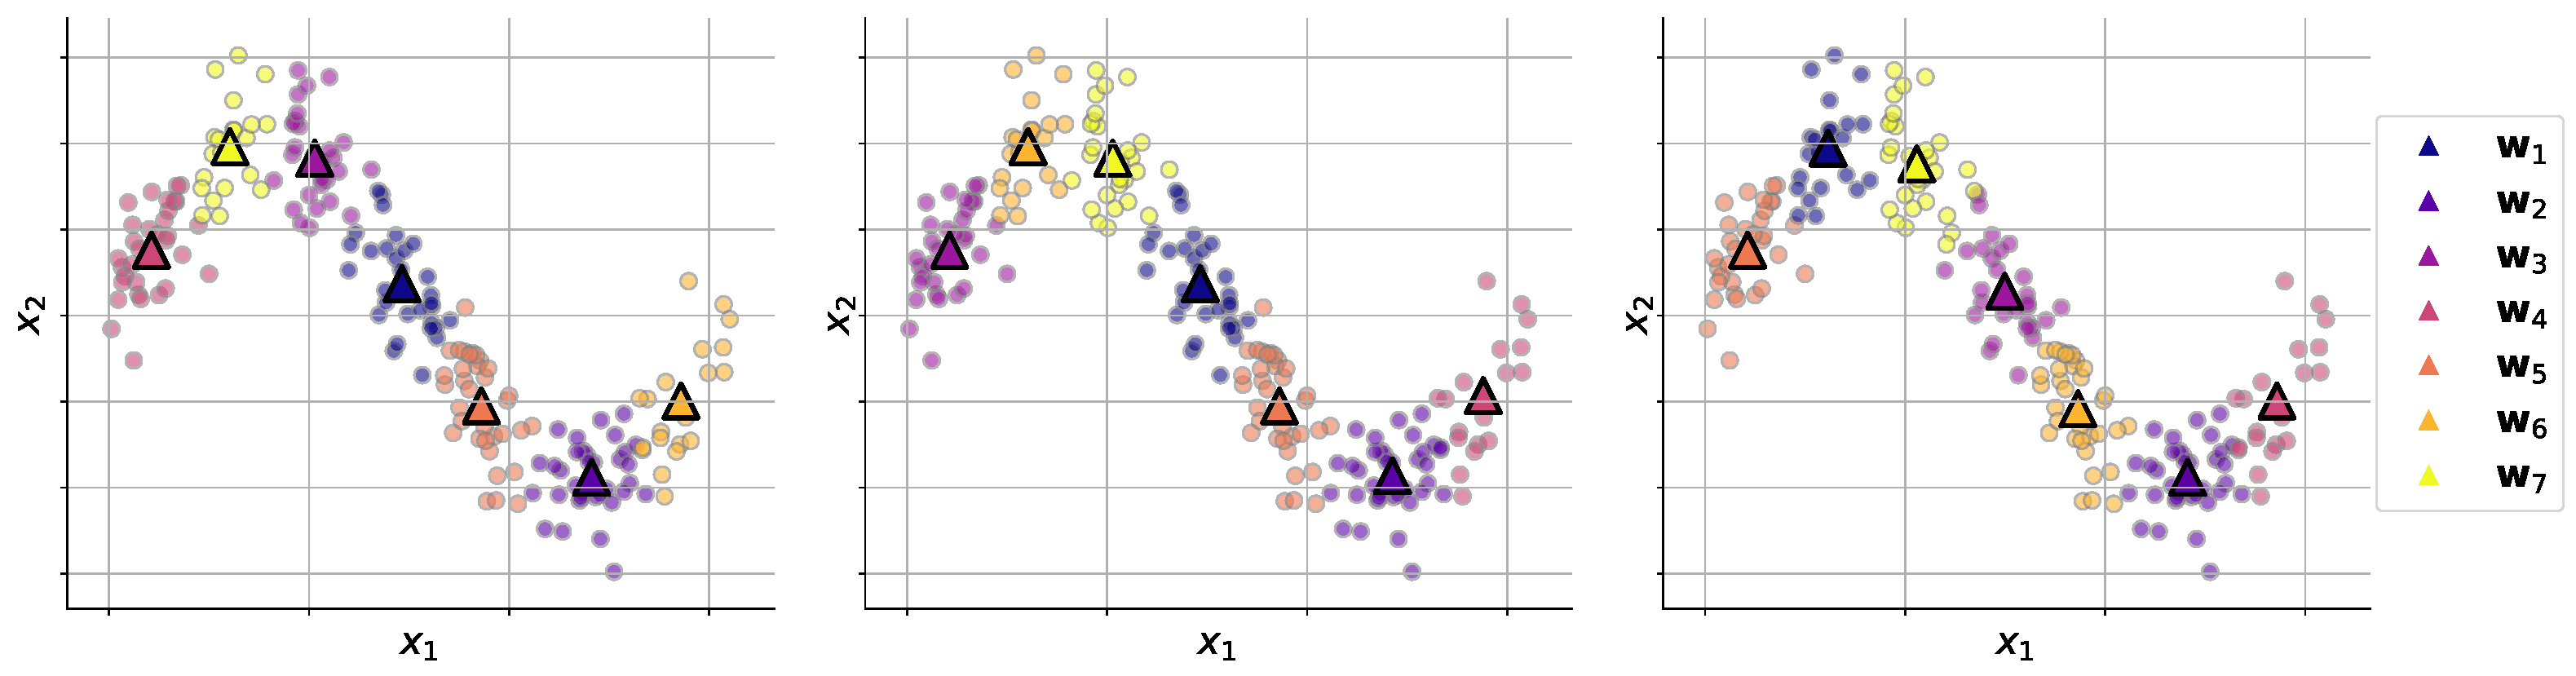
\includegraphics[trim=950 0 0 0,clip, width=0.9\textwidth]{img/sin_clustering}
	\notesonly{\captionof{figure}{A clustering solution with 7 prototypes.}}
\end{center}
\end{minipage}

\end{frame}

\begin{frame}{Multiple runs of K-means on the data}

\begin{center}
	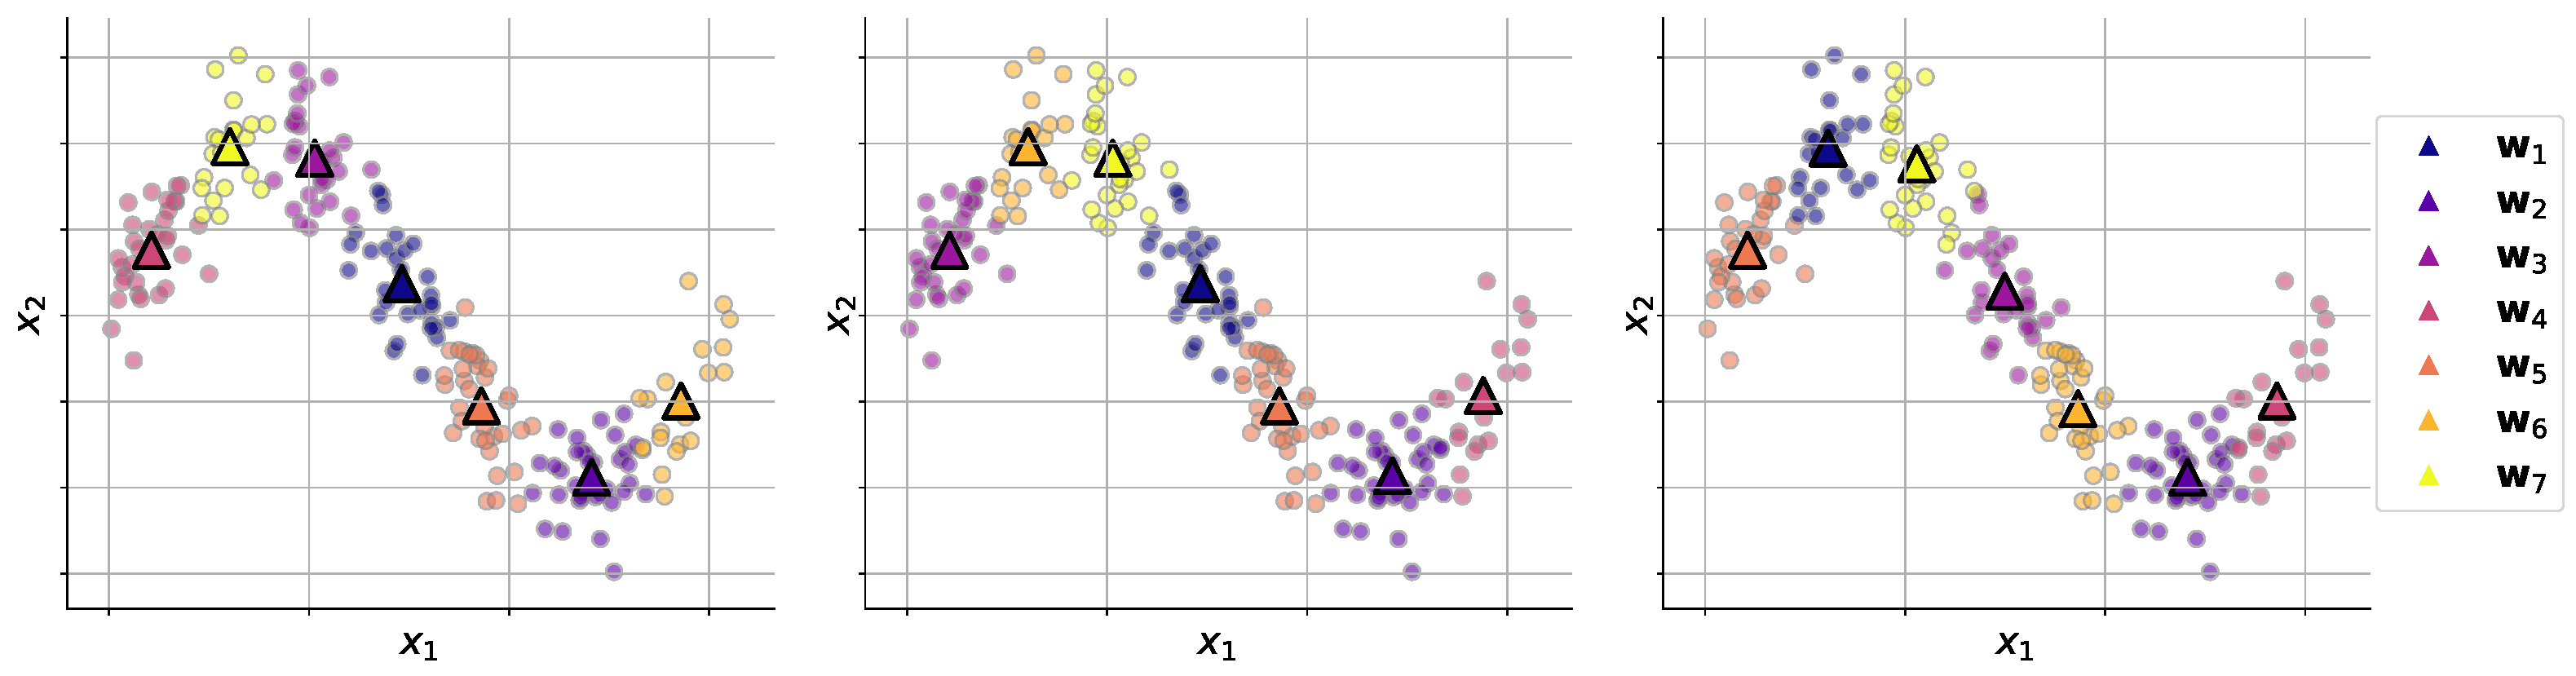
\includegraphics[width=0.95\textwidth]{img/sin_clustering}
	\captionof{figure}{Equivalent clustering solutions with 7 prototypes.}
\end{center}

\begin{itemize}
\item The clustering solutions are equivalent in that they are permutations of one another.
\item There is no ``order'' in the numbering of the cluster indices. The numbers don't reflect any topology about the clusters.
\end{itemize}

\end{frame}

\begin{frame}{Reflect topology by sorting the cluster indices}

Renumber the cluster indices by sorting the prototypes according to position along the horizonal axis.

\begin{center}
	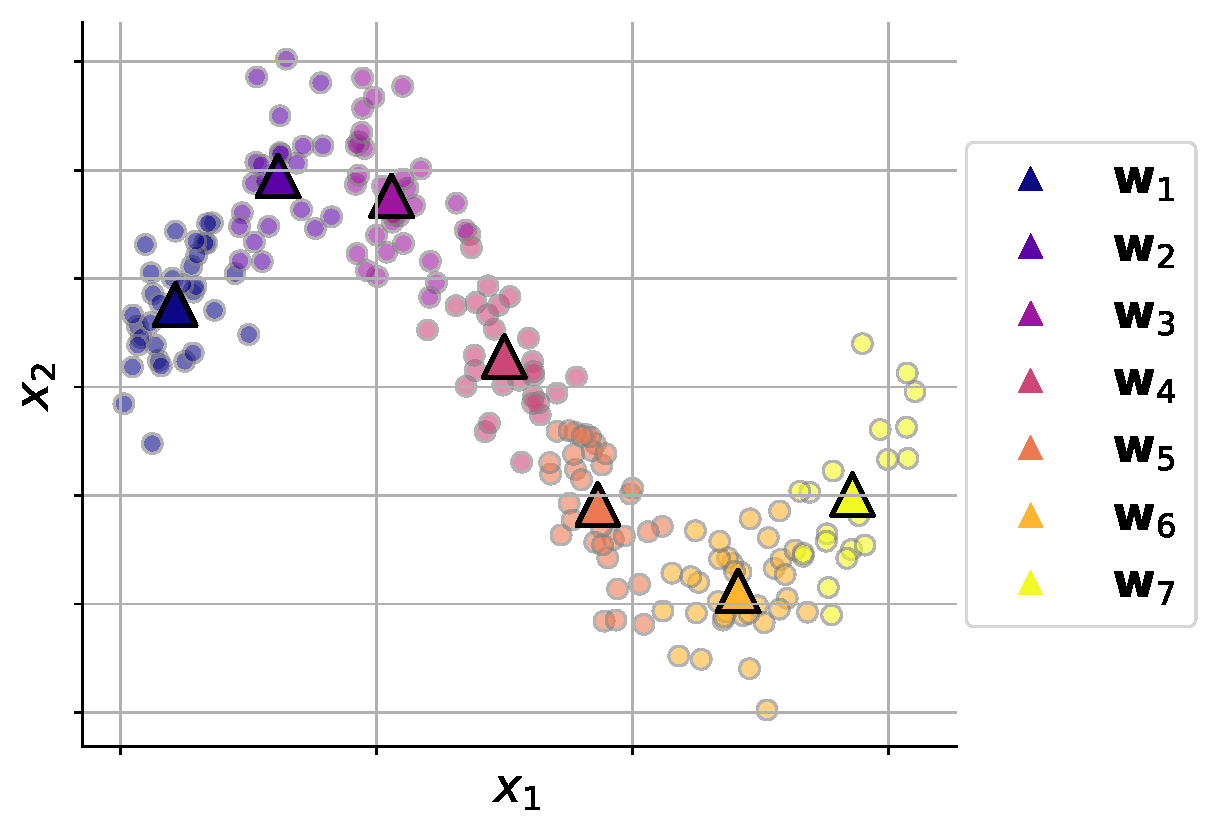
\includegraphics[width=0.5\textwidth]{img/sin_clustering_sorted}
	\notesonly{\captionof{figure}{Equivalent clustering solution with 7 prototypes that reflects some topology in the data.}}
\end{center}

$\vec w_{q}$ and $\vec w_{q+1}$ are neighbors in input space.

\end{frame}

\subsection{Motivation for clustering that preserves neighborhood}

\begin{frame}{\subsecname}

Recap from last time\\

\question{What does clustering give us?}
 
\begin{itemize}
\item[-] Discrete low-dimensional representation of data points.
\begin{equation}
\text{point}~\vec x \in \R^N \quad \longrightarrow \quad~\text{cluster index}~q \in \N
\end{equation} 
\item We will be able to describe the entire dataset by the partitions we've found that separate the clusters.
\item We'll draw relations between simple clustering and other algorithms (\textbf{embedding} algorithms, density estimation)
\end{itemize}

\end{frame}

\begin{frame}

\begin{block}{Embedding}

A low-dimensional representation of the data that is neighborhood preserving,
\begin{itemize}
\item[i.e.] account for local structure,
\item[e.g.] two points close in $N$-dim input space should remain close in the low-dimensional embedding space.
\end{itemize}

\end{block}

\end{frame}

\begin{frame}{A step towards manifold learning}

\begin{block}{The manifold: a handwavy explanation}

The space in which data resides that is possibly much lower than the $N$-dimensional space we observe it in.
It is a space in which we draw any insights from the data just as we try to do from the $N$-dim. observations (e.g. clustering, classifcation,...)

\end{block}

\pause

\begin{center}
	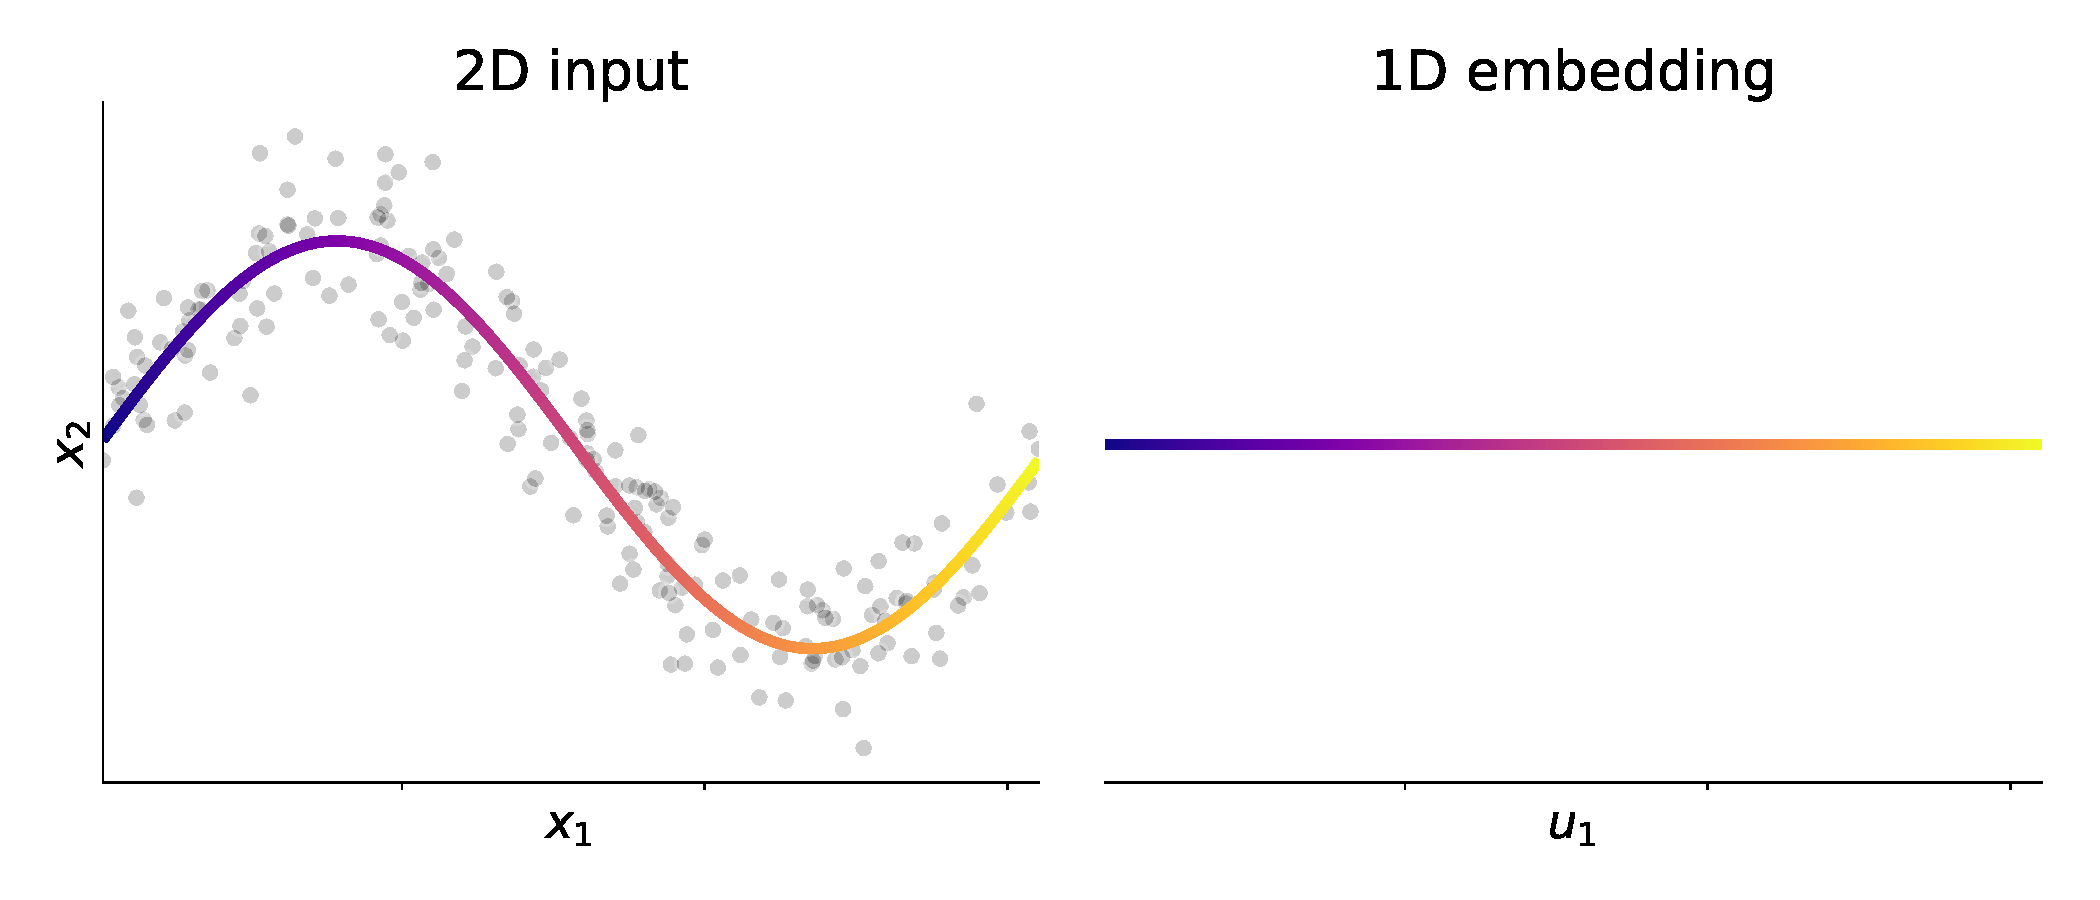
\includegraphics[width=0.8\textwidth]{img/sin_manifold}
	\captionof{figure}{A 1D embedding of the 2D sinusoidal curve}
\end{center}

\end{frame}

\begin{frame}{An ant's perspective}
\notesonly{Looking at data from the perspective of an \emph{ant}.}

\begin{center}
	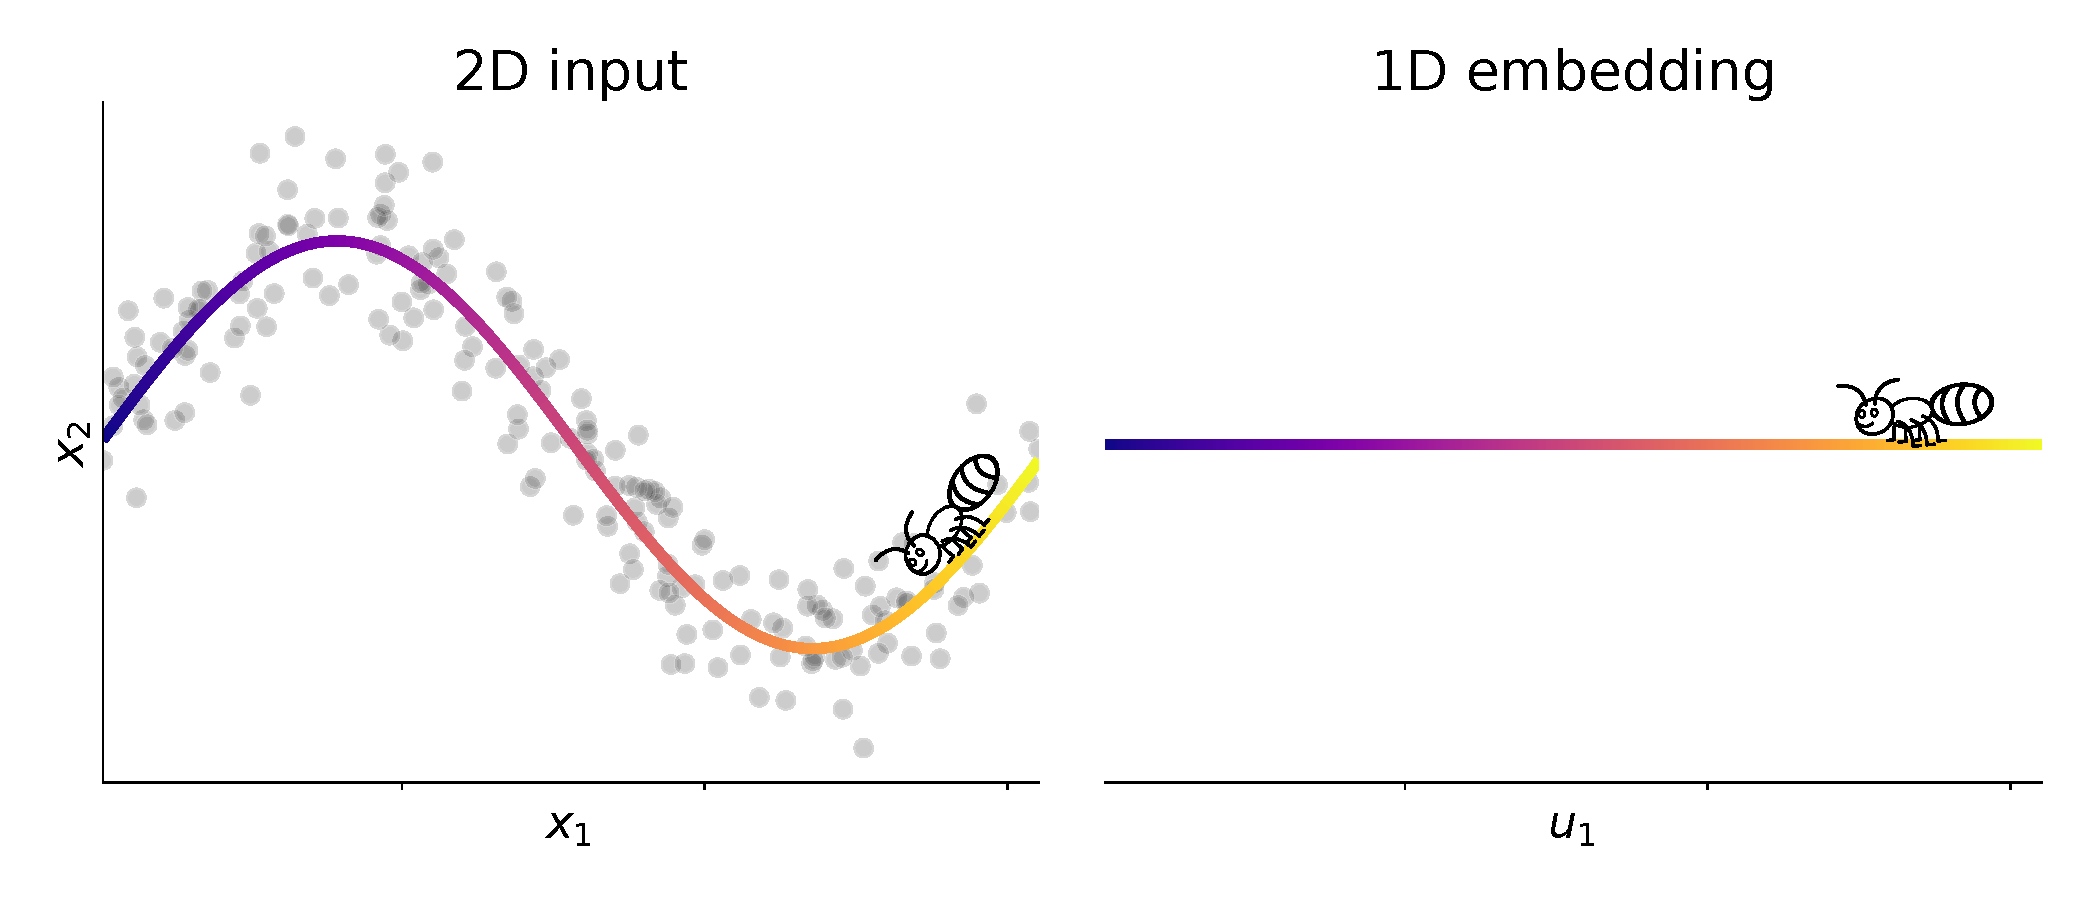
\includegraphics[width=0.9\textwidth]{img/sin_manifold_ant}
	\captionof{figure}{To the little ant, the sinusoid is just a 1D line. No turns, no elevation.}
\end{center}

\end{frame}

\begin{frame}

\slidesonly{
\begin{center}
	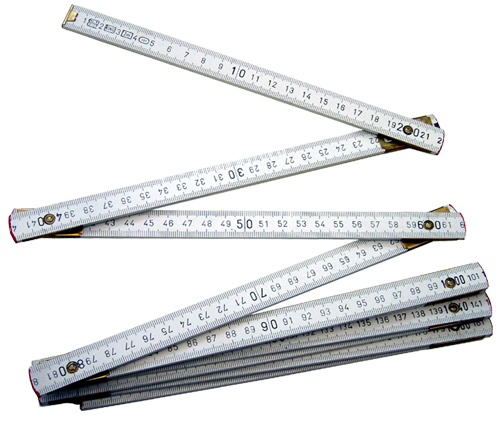
\includegraphics[width=0.3\textwidth]{img/Metre_pliant_500px}
	\captionof{figure}{Zollstock - Carpenter's rule}
\end{center}
}

\end{frame}

\begin{frame}{A discrete mapping}

\begin{center}
	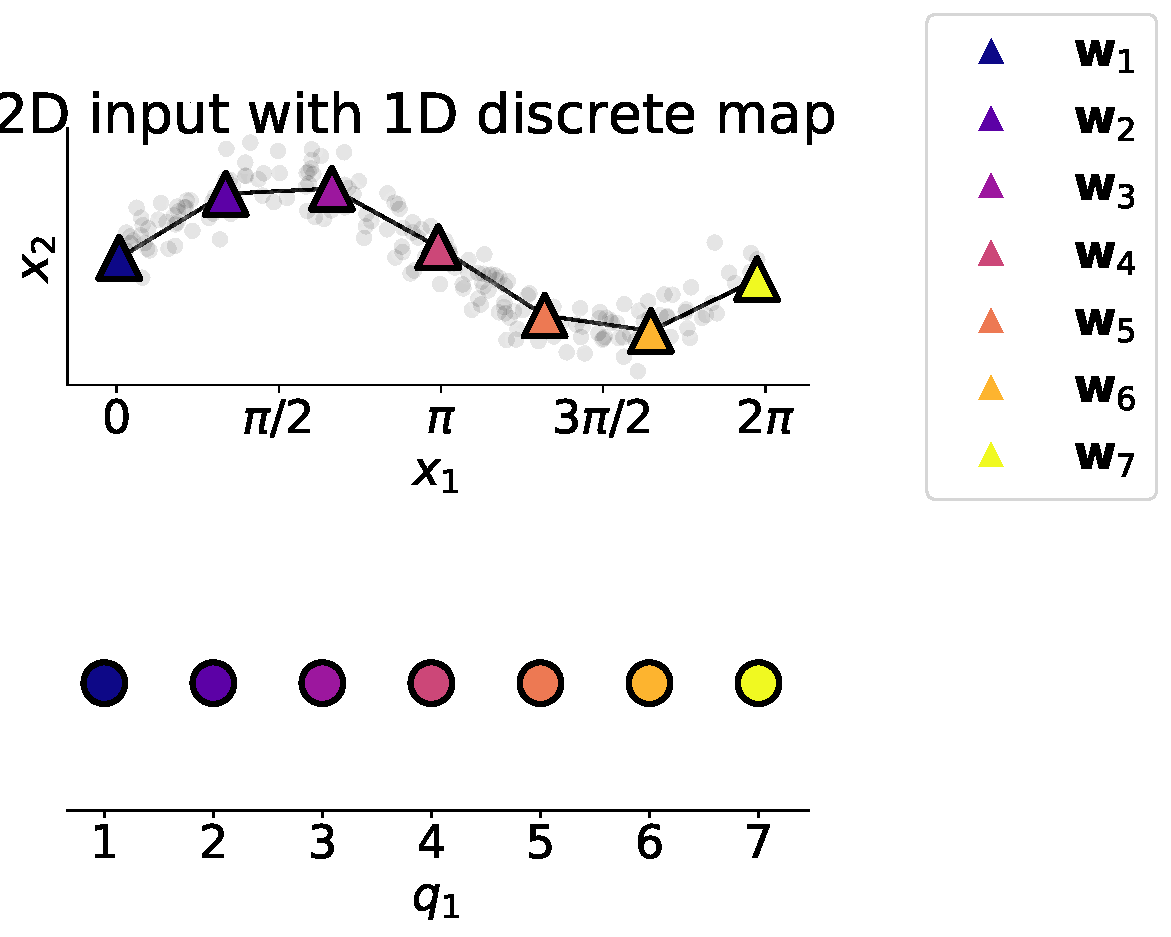
\includegraphics[width=0.6\textwidth]{img/sin_manifold_map}
	\captionof{figure}{2D input with a discrete mapping (e.g. SOM)}
\end{center}

\end{frame}
